\vspace{0.5cm}
\newline
\noindent\lecture{20}{21/12/2021}
\section{Caratterizzazione di un qubit superconduttivo}
Consideriamo un charge qubit nel limite TRANSMON in cui abbiamo $E_J\ll E_C$.  La piccola capacità si ottiene usando condensatori molto grandi, mentre posso controllare l'energia Josephson tramite: $E_J=\hbar\frac{I_o}{2e}$. Dove la corrente critica della giunzione è connessa all'energia di gap del superconduttore $\Delta(0)$ e alla resistenza a temperatura ambiente $R_n$:
\begin{equation*}
    I_0 = \frac{\pi \Delta(0)}{2eR_n}
\end{equation*}
Ad esempio, per l'alluminio, il gap è circa $\Delta(0) \approx 170 \,\mu eV$ e $R\sim10k\Omega$ per $I_0\sim0.010\mu A$.
Tutti questi parametri sono correlati e vanno scelti in modo da ottenere una frequenza caratteristica del qubit nell'ordine del GHz. Siccome abbiamo che $\omega_q=\sqrt{8E_JE_C}-E_C$, coi valori sopra menzionati arriviamo a $C\sim0.1pF$.
Supponiamo di avere un qubit simmetrico (in modo da poter controllare a piacimento la frequenza caratteristica) accoppiato capacitivamente a un risonatore LC (che può anche essere la rappresentazione di una CPW). Entrambe gli elementi sono portati a temperature prossime allo zero assoluto ($\sim 0.01K$) e il circuito complessivo è accoppiato all'esterno anch'esso tramite una capacità.
All'esterno è posto un circolatore in modo che sia possibile inviare un segnale al circuito "freddo" e analizzare poi il segnale riflesso. In particolare, ci aspettiamo dei cambiamenti di fase (90°) in corrispondenza dei picchi di risonanza dell'ampiezza (che potrebbero anch'essi venir analizzati, ma sono per definizione stretti).

\subsection{Identificazione delle frequenze caratteristiche}
La procedura per caratterizzare il qubit parte dal trovare le frequenze "libere" di cavità e qubit (non interagenti). Per misurare $\omega_c$ è sufficiente inviare dall'esterno frequenze ad elevata intensità in modo che "rompano" le caratteristiche superconduttive delle giunzioni Josephson del qubit. Analizzando le frequenze in arrivo con un VNA (\textit{Vector Network Analyzer}) siamo in grado di identificare il picco corrispondente alla frequenza della cavità.
Nel caso in cui il qubit non sia "inattivo" (dunque il segnale che inviamo è ora a bassa intensità), quanto abbiamo studiato della \textit{circuit QED} ci dice che il picco a $\omega_c$ viene "diviso" (nelle frequenze di transizione dei due diversi polarons) e spostato di $\pm \chi$ per l'effetto del \textit{Rabi splitting}.
Per identificare la frequenza del qubit $\omega_q$ stimolo il sistema con due diverse frequenze: una la scelgo fra quelle appena trovate della cavità in interazione e la seconda la vario alla ricerca di $\omega_q$. Fintanto che la seconda sorgente non identifica la frequenza del qubit, la prima (di cui continuo a osservare il riflesso col VNA) mi identificherà una risonanza, ma quando la seconda frequenza ecciterà il qubit, anche la cavità cambierà frequenza di risonanza e col VNA vedrò che non siamo più su un picco.
Così abbiamo identificato tutte le frequenze caratteristiche necessarie.

\subsection{Controllo e misura (omodina e eterodina)}

Per controllare e misurare il qubit utilizzeremo nuovamente dei mixer IQ (nello schema detto omodina o nell'eterodina).
L'idea generale è di mandare un medesimo segnale attraverso il qubit (nella porta RF) e non-attraverso il qubit (nella porta LO) a un IQ mixer: i due segnali si mescoleranno in modo differente a seconda dello stato del qubit.
Il qubit avrà due frequenze di risonanza (corrispondenti a $\ket g$ e $\ket e$), generalmente si utilizza una frequenza intermedia per la misurazione (la si sceglie sperimentalmente). Il qubit deve essere alla temperatura minore possibile in modo da minimizzare l'errore sul segnale in uscita (che viene peggiorato da fluttuazioni sul numero di fotoni). Viene anche posizionato, dopo il qubit, un amplificatore parametrico che "riesce" ad amplificare il segnale senza introdurre rumore (con una sorta di misurazione QND).
Il segnale inviato al qubit viene, in realtà, modificato tramite un IQ mixer prima di raggiungere il qubit stesso in modo da essere formato e limitato nel tempo nel modo migliore, per massimizzare la \textit{fidelity} della misurazione.
Lo spostamento delle frequenze è dominato dal parametro $\chi = \frac{g^2}{\Delta}$. La migliore separazione fra esse è ottenuta con il fattore di merito $Q=\omega_c / k$ con $k$ che è la vita media della risonanza nella cavità e vale anche $\chi = k/2$.
Supponiamo di poter scrivere il segnale in uscita come (RO indica \textit{redout}):
\begin{equation*}
    s(t)=A_{RO}\cos(\omega_{RO}t+\theta_{RO})
\end{equation*}
Dove $\theta$ è lo sfasamento che il segnale subisce attraversando il qubit.
Possiamo riscriverla anche come:
\begin{equation*}
    s(t)=\Re{A_{RO}e^{i\theta_{RO}}e^{i\omega_{RO}t}}
\end{equation*}
Il secondo termine esponenziale corrisponde a una rotazione nel piano complesso, mentre il primo termine ($A_{RO}e^{i\theta_{RO}}$) in elettromagnetismo è detto fasore e possiamo riscriverlo come:
\begin{equation*}
    A_{RO}e^{i\theta_{RO}}=A_{RO}\cos(\theta_{RO})+iA_{RO}\sin(\theta_{RO})=I+iQ
\end{equation*}
Abbiamo trovato nuovamente le due quadrature dell'onda.
Passiamo adesso a una configurazione del circuito leggermente diversa (e più generale). I due segnali che vanno all'IQ mixer non provengono più dal medesimo generatore, ma da due generatori diversi. Al gate LO verrà inviata una frequenza oscillante $y(t)=A_{LO}\cos(\omega_{LO}t)$, mentre non cambierà l'input della porta RF (col segnale che attraversa il qubit). 
Il mixer IQ produrrà un output in I proporzionale a:
\begin{equation*}
   I(t)\propto\cos((\theta_{RO}-\omega_{LO})t+\theta_{RO})+\cos((\omega_{RO}+\omega_{LO})t+\theta_{RO})
\end{equation*}
Abbiamo, in generale, che le due frequenze $\omega_{RO}$ e $\omega_{LO}$ sono molto simili, perciò il primo termine sarà a bassa frequenza, mentre il secondo ad altra frequenza. Applicando un filtro passa-basso potremo selezionare il solo primo termine.
Per l'output Q otteniamo in modo analogo:
\begin{equation*}
    Q (t) \propto \sin \left( \left( \omega_{RO} - \omega_{LO} \right) t + \theta_{RO} \right)
\end{equation*}
Nel caso in cui i due segnali provengano dal medesimo generatore (come stavamo vedendo prima) siamo nel cosiddetto schema di omodina. Otteniamo, in questo modo: $Q=\cos(\theta_{RO})$, $I=\sin(\theta_{RO})$. Abbiamo, dunque, che il fasore nel piano complesso è descritto da $\theta = \arctan \frac{Q}{I}$ e $A = \sqrt{Q^2 + I^2}$. Tale fasore rimarrà pressoché invariato a meno di un cambio di stato del qubit che porterà a una leggera modifica dell'ampiezza e a una grande modifica dell'angolo. In partenza avremo un errore non trascurabile sia su I che su Q (errori uguali) e sarebbe difficile distinguere i due risultati. Amplificando un un operazionale classico, poi, peggioreremmo la situazione amplificando il rumore stesso e aggiungendone ancora dell'altro. La soluzione sta nell'usare un amplificatore parametrico che riesce a indirizzare tutto l'errore su una quadratura e non sull'altra, in questo modo i due diversi fasori rimangono altamente distinguibili.
Se invece, i due generatori non sono uguali (eterodina: è un po' più complessa, ma quasi necessaria nel caso in cui si vogliano misurare e controllare diversi qubit) le due frequenze non si cancellano in I e Q in uscita. Otterremo una frequenza intermedia $\omega_{IF} = \omega_{RO} - \omega_{LO}$. Il fasore, dunque, rimarrà in rotazione (benchè a bassa frequenza) nel piano complesso dato da I e Q (Z è il fasore):
\begin{equation*}
    Z_{IF}(t)=Ae^{i\omega_{IF}t}e^{i\theta{IF}}
\end{equation*}
Dovremo moltiplicare il segnale per una rotazione uguale e contraria (tendenzialmente lo faremo via software) in modo da cancellare il termine spurio rotatorio.
Abbiamo adesso tutti gli elementi necessari per eseguire una misura di Rabi. La configurazione del circuito è più complessa nel caso reale (dove abbiamo anche bisogno di un segnale di \textit{drive}) con $\omega_q$ ed è illustrata in figura.
\begin{figure}[H]
    \centering
    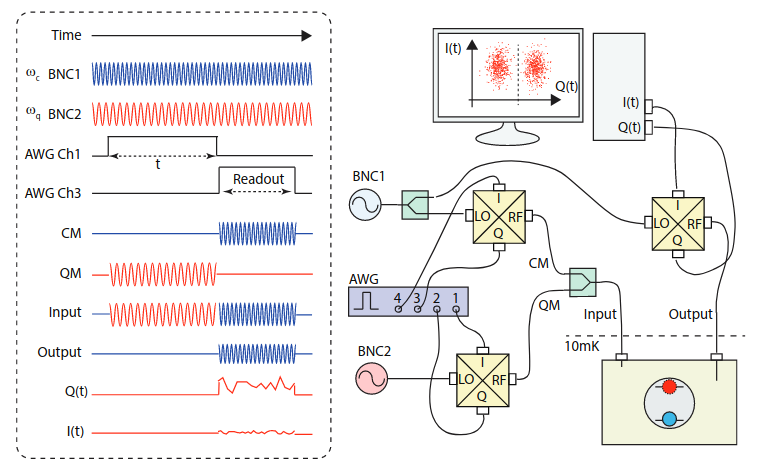
\includegraphics[width=\textwidth]{images/rabi_measur_heterodyne.png}
    \caption{Rabi measurement: The sequence for the measurement of Rabi oscillations and the typical
room temperature circuitry are shown. \url{https://arxiv.org/pdf/1904.09291.pdf}}
\end{figure}
La probabilità di misurare lo stato eccitato dipende dalla durata $t$ del segnale in ingresso che va in oscillazione di Rabi con il qubit:
\begin{equation*}
    P_{\ket e}= \frac{A^2}{A^2 + \Delta^2} \sin^2 \left( \frac{\sqrt{A^2 + \Delta ^ 2}}{2}t \right)
\end{equation*}
La scelta di $t$ deve essere chiaramente fatta in modo da massimizzare la probabilità di misura corretta.
Essendo una misura probabilistica, comunque, è necessario ripetere le operazioni di misura diverse volte, in modo da arrivare al risultato corretto a meno di soli errori statistici. 
Bisogna stare attenti, tuttavia, che dopo un certo tempo il qubit "perde" il suo stato per rilassamento e \textit{dephasing}.

\subsection{Misura di T1 e T2}
Per misurare il tempo di rilassamento (ovvero il tempo per cui $\ket 1$ decade in $\ket 0$) è sufficiente portare il qubit nello stato eccitato ed eseguire misure dopo tempi diversi del qubit stesso. Vedremo che la probabilità di trovare il qubit nello stato eccitato diminuirà in modo esponenziale con una costante di tempo (identificabile tramite \textit{fitting}) pari a $T_1$.
Per il tempo di \textit{dephasing}, invece, utilizziamo una misura di Ramsey (simile a quella di cui abbiamo discusso nel caso di atomi usati come sonde per misurare lo stato di una cavità).
L'idea è di inviare, separati da un certo tempo $t$, due impulsi $\pi/2$ (rotatori). Se fra le due rotazioni non avviene \textit{dephasing}, alla fine misureremo lo stesso stato iniziale. Ripetendo l'esperimento per diversi $t$ otterremo nuovamente un esponenziale decrescente con $T_2$. 
In realtà, nella pratica, si usa una frequenza di drive sfasata in partenza rispetto alla frequenza di risonanza. La curva finale non sarà un esponenziale, ma una sinusoide modulata da un'esponenziale. Ciò viene fatto per evitare che errori nella modulazione passino inosservati e portino a $T_2$ poco precisi.

\subsubsection{Tomografia}
Fino ad ora abbiamo considerato misure solo lungo l'asse z, ma idealmente ci piacerebbe studiare uno stato qualsiasi nello spazio tridimensionale di Bloch.
Quello che si fa usualmente è di triplicare uno stato su tre diversi qubit: il primo viene misurato lungo l'asse z, gli altri ruotati adeguatamente e poi misurati. In questo modo è possibile misurare una generica sovrapposizione di stati.